\section{Progettazione Concettuale}
	
	\subsection{Strategia di Progetto}
		\emph{Top-down} per la realizzazione dello schema ad un adeguato livello di raffinamento. 
						
		{\color{red}{Questa sezione va ampliata e corretta}}
		
	\subsection{Individuazione dello Scheletro dello Schema ER}
		
		Dalle specifiche che abbiamo formulato risulta che uno dei punti fondamentali da affrontare è quello della memorizzazione dei preventivi emessi dall'attività.
		Ad ogni \emph{Prestazione} effettuata, corrisponde un \emph{Preventivo} precedentemente emesso.
		
		\begin{figure}[H]
			\centering
			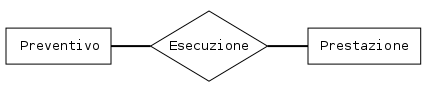
\includegraphics[width=9cm]{images/diagrams/preventivo_prestazione.png}
		\end{figure}
		
		Alla formulazione di ogni preventivo, si fa una stima dei componenti che si reputa saranno necessari per eseguire la prestazione preventivata. Non sempre tale previsione è completamente completamente esatta, generalmente i componenti effettivamente utilizzati in una prestazione sono diversi da quelli previsti in un preventivo.
		L'associazione tra i \emph{Componenti} e il \emph{Preventivo} risulta immediata.
		
		\begin{figure}[H]
			\centering
			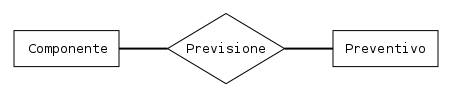
\includegraphics[width=9cm]{images/diagrams/preventivo_componente.png}
		\end{figure}
		
		Prima di esplicitare l'associazione tra le prestazioni eseguite ed i componenti effettivamente utilizzati, affrontiamo la questione degli ordini e del magazzino.
		
		L'acquisto di articoli presso un fornitore è formalizzato in un ordine, il quale, come da specifiche, è organizzato in più forniture, ovvero insiemi di articoli di uno stesso componente.
		Ad un \emph{Ordine} sono associate una o più \emph{Forniture} di articoli, ognuna delle quali fanno riferimento ad un \emph{Componente}.
		
		\begin{figure}[H]
			\centering
			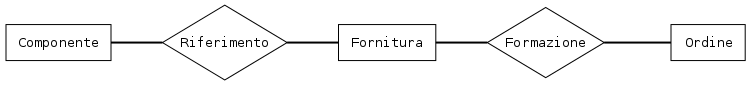
\includegraphics[width=11.5cm]{images/diagrams/componente_ordine.png}
		\end{figure}
		
		Il magazzino, nella realtà, è composto dai vari articoli acquistati che sono in attesa di essere utilizzati. La classificazione degli articoli avviene, in primo luogo per componente, in secondo luogo per fornitura d'appartenenza. Non vi è così il bisogno di registrare ogni articolo individualmente, ma basterà riferirsi alle relative forniture.
		Il \emph{Magazzino} è una composizione di \emph{Forniture} i cui articoli sono depositati in attesa di essere utilizzati.
		
		\begin{figure}[H]
			\centering
			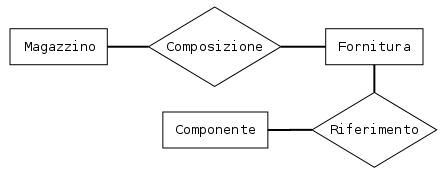
\includegraphics[width=9cm]{images/diagrams/magazzino_fornitura.png}
		\end{figure}
		
		Per identificare con precisione quali articoli sono stati utilizzati per l'esecuzione di una prestazione, sarà sufficiente riferirsi alla fornitura relativa agli stessi. Da questa si ottengono le informazioni sul componente (quindi il prezzo di vendita e il tempo di validità) e sulla data d'acquisto.
		Ad ogni utilizzo, si provvederà ad aggiornare le quantità rimanenti degli articoli delle forniture utilizzate.
		Per l'esecuzione di una \emph{Prestazione} si possono utilizzare gli articoli di più \emph{Forniture}.
		
		\begin{figure}[H]
			\centering
			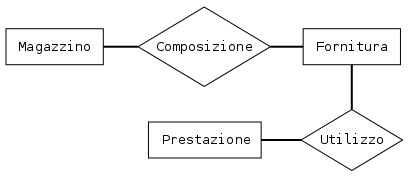
\includegraphics[width=9cm]{images/diagrams/prestazione_fornitura.png}
		\end{figure}
		
		Passiamo alla questione degli operatori. Una prestazione viene eseguita da uno o più operatori. Di ogni operatore si vuole tener traccia dei turni di lavoro effettuati.
		Alla \emph{Prestazione}, saranno associati uno o più \emph{Operatori} ad ognuno dei quali sono associati i relativi \emph{Turni} di lavoro.
		
		\begin{figure}[H]
			\centering
			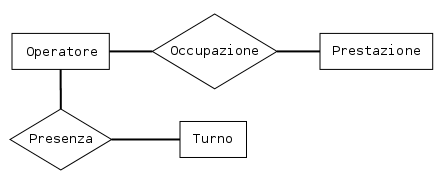
\includegraphics[width=9cm]{images/diagrams/operatore_turno_prestazione.png}
		\end{figure}
		
		Occupiamoci ora delle zone periferiche dello schema. Un preventivo viene effettuato quando un cliente richiede un intervento alla propria auto.
		Ad ogni \emph{Cliente} vengono associate una o più \emph{Autovetture}. Ogni \emph{Preventivo} si riferisce ad una specifica \emph{Autovettura}.
		
		\begin{figure}[H]
			\centering
			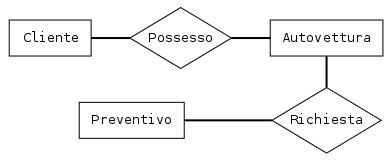
\includegraphics[width=9cm]{images/diagrams/cliente_autovettura_preventivo.png}
		\end{figure}
		
		Ogni \emph{Ordine} viene effettuato presso un \emph{Fornitore}.
		
		\begin{figure}[H]
			\centering
			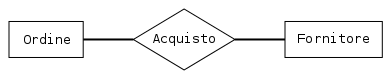
\includegraphics[width=9cm]{images/diagrams/ordine_fornitore.png}
		\end{figure}
		
		Notiamo che \emph{Cliente} rappresenta sia \emph{Privati} che \emph{Aziende} (rispettivamente, clienti non dotati di partita iva e clienti dotati di partita iva).
		
		\begin{figure}[H]
			\centering
			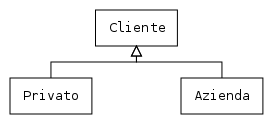
\includegraphics[width=7.5cm]{images/diagrams/cliente.png}
		\end{figure}
		
		Inoltre \emph{Clienti}, \emph{Fornitori} ed \emph{Operatori} possono essere generalizzati dall'entità \emph{Persona}.
		
		\begin{figure}[H]
			\centering
			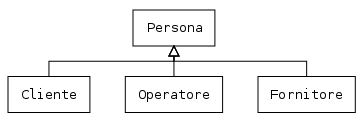
\includegraphics[width=10cm]{images/diagrams/persona.png}
		\end{figure}
		
		Ad ogni \emph{Persona} saranno associati uno o più \emph{Recapiti}.
		
		\begin{figure}[H]
			\centering
			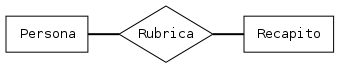
\includegraphics[width=9cm]{images/diagrams/persona_recapito.png}
		\end{figure}
		
		Possiamo concludere lo sviluppo della struttura del diagramma ER affrontando la questione delle transazioni. Avviene una \emph{Transazione} ogni volta che viene versato un acconto per un \emph{Preventivo}, ogni volta che viene saldata la \emph{Fattura} di una \emph{Prestazione}, ogni volta che viene pagato un \emph{Ordine} ed ogni volta che viene pagato il salario di un \emph{Operatore}.
		
		\begin{figure}[H]
			\centering
			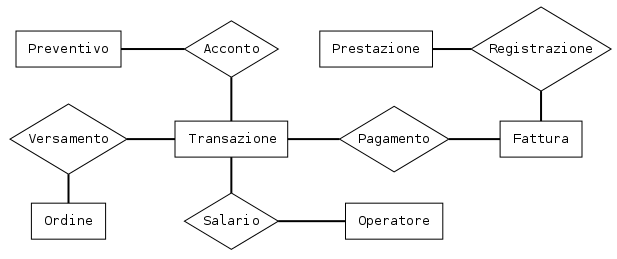
\includegraphics[width=12cm]{images/diagrams/transazione.png}
		\end{figure}
			
		Il diagramma in figura \ref{fig:scheletro_er} rappresenta lo scheletro dello schema ER.
		
		\begin{sidewaysfigure}
			\centering
			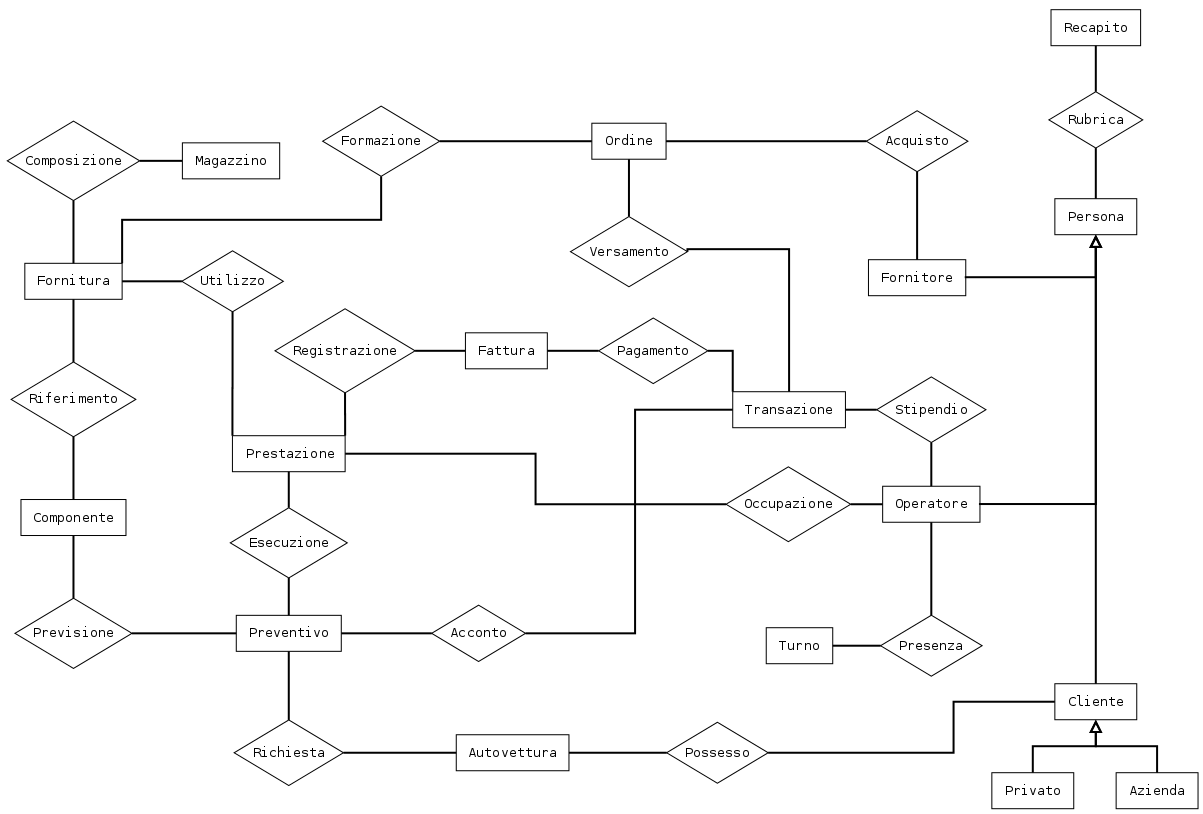
\includegraphics[width=20cm]{images/diagrams/schema.png}
			\caption{Scheletro del diagramma ER}
			\label{fig:scheletro_er}
		\end{sidewaysfigure}
	
	\subsection{Sviluppo delle Componenti dello Schema}
	
		Ottenuto lo scheletro generale del diagramma ER procediamo ad esplicitare, delle entità principali, l'insieme degli attributi che ognuna di esse possiede.
		Una volta sviluppati gli attributi delle entità principali svilupperemo le relationship che le legano, raggruppandole tra loro sulla falsariga dei modelli elaborati allo step precedente.
		
		Gli attributi di ogni entità derivano ovviamente dall'analisi dei requisi della base di dati, quindi le successive sezioni si limitano a presentare graficamente i successivi raffinamenti sulle componenti dello schema ER, con l'aggiunta di eventuali descrizioni per integrare ciò che non era stato già detto.
		Per una lettura più accurata e rigorosa di tali diagrammi si rimanda alla consultazione della documentazione di supporto (Dizionario dei Dati alla sezione \ref{sec:data_dict} e Regole Aziendali \ref{sec:business_rules}).
		
		\begin{description}
			\item[NB]
				Ogni generalizzazione effettuata è da considerarsi totale.
		\end{description}
		
		\subsubsection{Persona}
		
			In figura \ref{fig:persona} troviamo lo sviluppo degli attributi dell'entità \emph{Persona} e delle relative entità che la estendono.
						
			\begin{figure}[H]
				\centering
				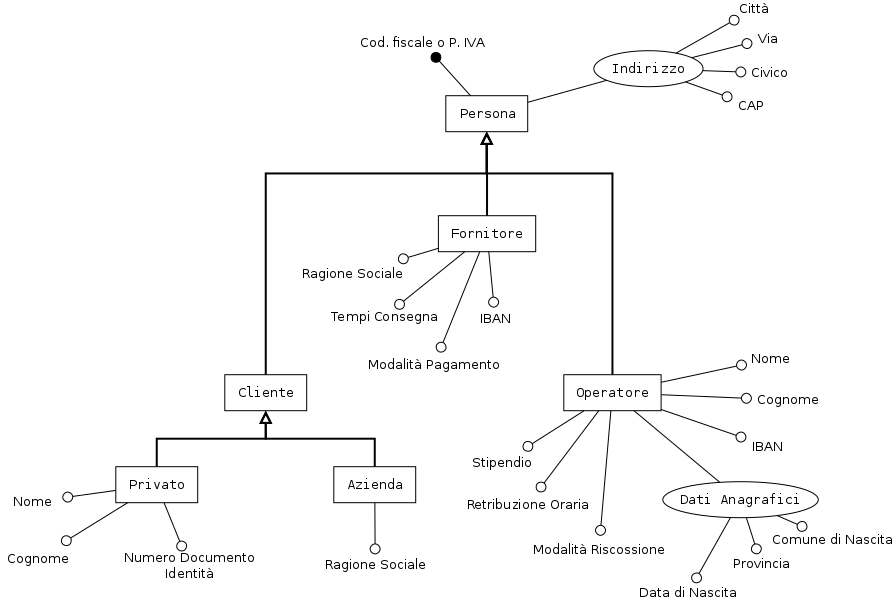
\includegraphics[width=12cm]{images/finitures/persona.png}
				\caption{Sviluppo di Persona}
				\label{fig:persona}
			\end{figure}
			
			Di ogni \emph{Persona} coinvolta nelle attività dell'azienda, suddivisibili in \emph{Clienti}, \emph{Fornitori} ed \emph{Operatori}, è necessario memorizzare all'interno della base di dati il codice fiscale e l'indirizzo di riferimento.
		
		\subsubsection{Autovettura}
			
			Continuiamo con gli attributi che caratterizzano l'entità \emph{Autovettura} (Diagramma in figura \ref{fig:autovettura})
			
			\begin{figure}[H]
				\centering
				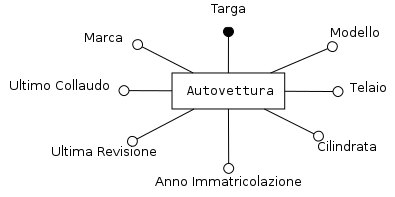
\includegraphics[width=9cm]{images/finitures/autovettura.png}
				\caption{Sviluppo dell'entità Autovettura}
				\label{fig:autovettura}
			\end{figure}
			
		\subsubsection{Preventivo}
		
			In figura \ref{fig:preventivo}, il diagramma espone gli attributi dell'entità \emph{Preventivo}.
			
			\begin{figure}[H]
				\centering
				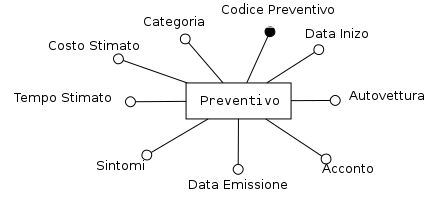
\includegraphics[width=9cm]{images/finitures/preventivo.png}
				\caption{Sviluppo dell'entità Preventivo}
				\label{fig:preventivo}
			\end{figure}
		
		\subsubsection{Prestazione}
			
			Gli attributi dell'entità \emph{Prestazione} vengono esplicitati dal diagramma in figura \ref{fig:prestazione}.
		
			\begin{figure}[H]
				\centering
				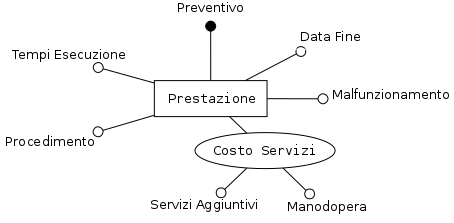
\includegraphics[width=9cm]{images/finitures/prestazione.png}
				\caption{Sviluppo dell'entità Prestazione}
				\label{fig:prestazione}
			\end{figure}
		
		\subsubsection{Componente}
			
			Nel diagramma in figura \ref{fig:componente} troviamo l'entità \emph{Componente} ed i relativi attributi.
			
			\begin{figure}[H]
				\centering
				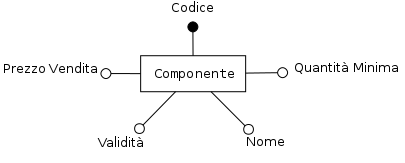
\includegraphics[width=9cm]{images/finitures/componente.png}
				\caption{Sviluppo di Componente}
				\label{fig:componente}
			\end{figure}
		
		\subsubsection{Altre entità di base}
		
		\subsubsection{Raffinamenti Successivi}
			
			Esplicitati gli attributi delle principali entità, procediamo a legarle tra loro sviluppando le relationship ed alcune entità minori.
			
			Ripercorrendo i passi dello sviluppo dello scheletro del diagramma ER, partiamo dalle relationship che legano le entità \emph{Cliente}, \emph{Autovettura}, \emph{Preventivo} (diagramma in figura \ref{fig:cliente_autovettura_preventivo}).			
		
			\begin{figure}[H]
				\centering
				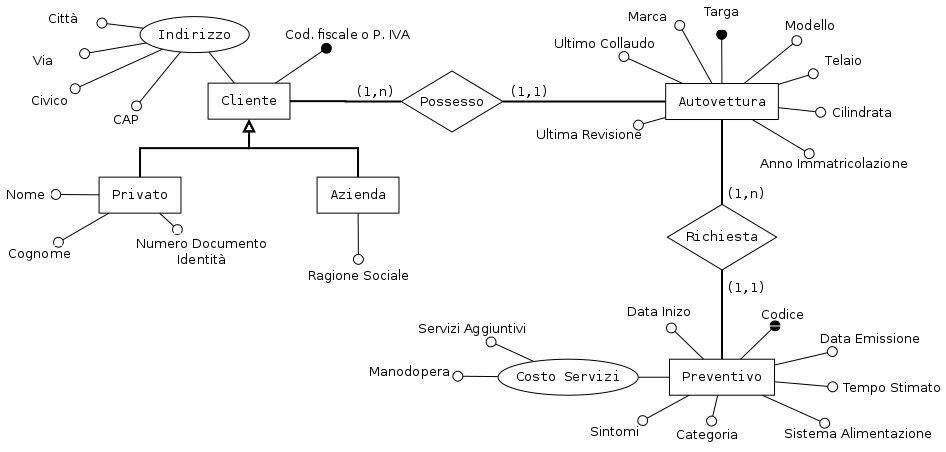
\includegraphics[width=13cm]{images/finitures/cliente_autovettura_preventivo.png}
				\caption{Sviluppo di Cliente, Autovettura, Preventivo}
				\label{fig:cliente_autovettura_preventivo}
			\end{figure}
			
			Chiaramente ad ogni cliente registrato, saranno associate una o più autovetture di sua propiertà. Ad ogni autovettura saranno associati uno o più preventivi di interventi riferiti all'autovettura stessa.
			
			Se l'intervento preventivato viene realizzato, al preventivo sarà associata una ed una sola prestazione. La stipulazione del preventivo non è vincolante nei confronti del cliente, quindi non è vero che ad ogni preventivo corrisponde una prestazione.
			
			\begin{figure}[H]
				\centering
				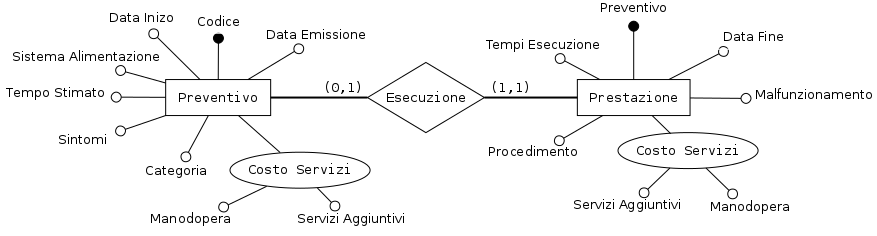
\includegraphics[width=13cm]{images/finitures/preventivo_prestazione.png}
				\caption{Sviluppo delle componenti di Preventivo e Prestazione}
				\label{fig:preventivo_prestazione}
			\end{figure}
		
		\subsubsection{Preventivo e Componente}
		
			\begin{figure}[H]
				\centering
				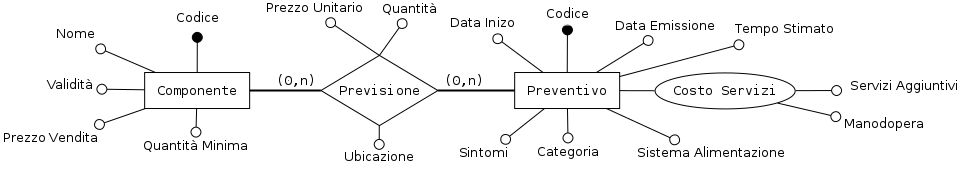
\includegraphics[width=11.5cm]{images/finitures/preventivo_componente.png}
				\caption{Sviluppo di Preventivo e Componente}
				\label{fig:preventivo_componente}
			\end{figure}
		
		\subsubsection{Magazzino ed Ordine}
		
			\begin{figure}[H]
				\centering
				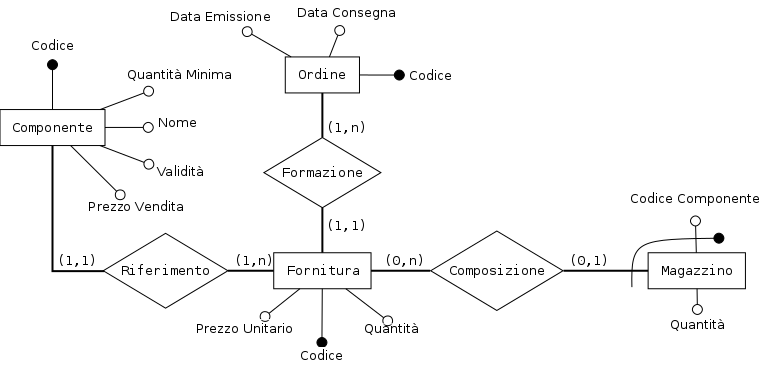
\includegraphics[width=11.5cm]{images/finitures/componente_fornitura_ordine_magazzino.png}
				\caption{Sviluppo delle componenti di Magazzino, Ordine, Componente, Fornitura}
				\label{fig:componente_fornitura_ordine_magazzino}
			\end{figure}
		
		\subsubsection{Fornitore}
			
			\begin{figure}[H]
				\centering
				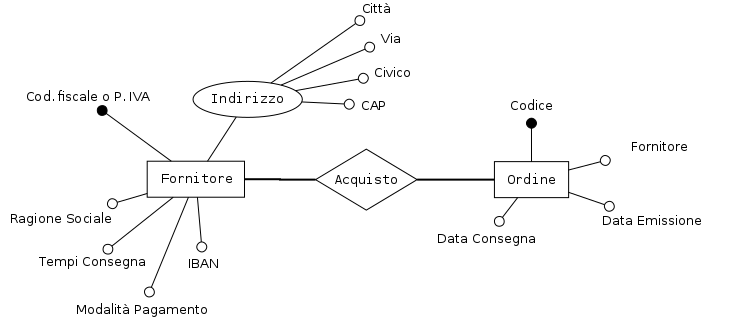
\includegraphics[width=11.5cm]{images/finitures/ordine_fornitore.png}
				\caption{Sviluppo delle componenti di Fornitore}
				\label{fig:ordine_fornitore}
			\end{figure}
			
		\subsubsection{Prestazione e Fornitura}
			
			\begin{figure}[H]
				\centering
				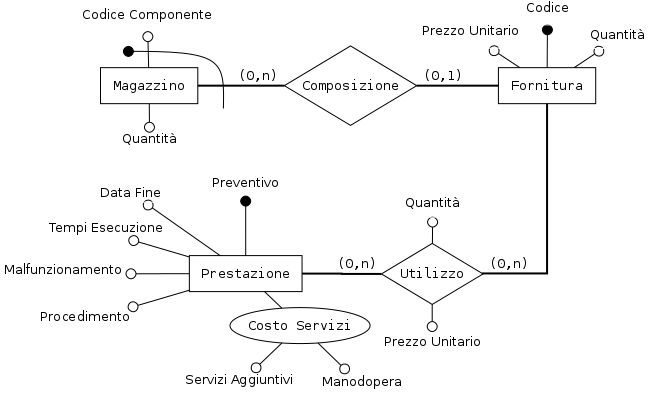
\includegraphics[width=11.5cm]{images/finitures/prestazione_fornitura.png}
				\caption{Sviluppo}
				\label{fig:ordine_fornitore}
			\end{figure}
		
		\subsubsection{Operatore}
		
			\begin{figure}[H]
				\centering
				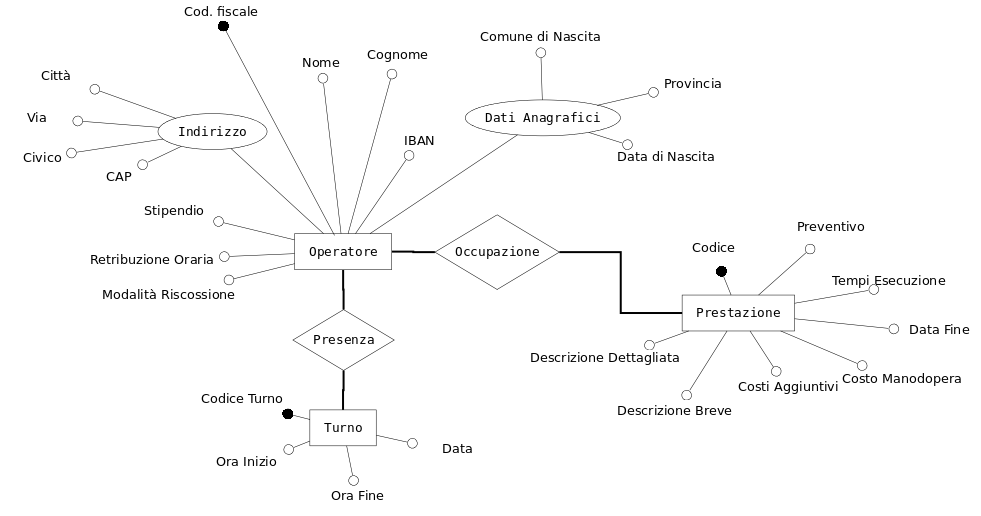
\includegraphics[width=11.5cm]{images/finitures/operatore_turno_prestazione.png}
				\caption{Sviluppo di Operatore, Turno, Prestazione}
				\label{fig:operatore_turno_prestazione}
			\end{figure}
			

	\subsection{Analisi Qualitativa dello Schema ER}
	
	% Sezione documentativa della progettazione concettuale
	\subsection{Dizionario dei Dati}
	\label{sec:data_dict}
		
		\subsubsection{Entità}
		\label{sec:entities}
		
			\begin{longtable}{| p{2.5cm} | p{4.5cm} | p{2cm} | p{2.5cm} |}
				\hline
				
					\textbf{Nome} & \textbf{Descrizione} & \textbf{Attributi} & \textbf{Identificatore} \\ \hline
					
					Nome entità & 
					Descrizione entità & 
					Attributi entità & 
					Identificatore entità
					\\
					
				\hline
			\end{longtable}

		\subsubsection{Relazioni}
		\label{sec:relationships}
	
	\subsection{Regole Aziendali}
	\label{sec:business_rules}
	
		\subsubsection{Regole di Vincolo}
		\subsubsection{Regole di Derivazione}
